\section{Пример секции}

\begin{definition}
	Мир, это когда нет войны
\end{definition}

\begin{corollary}
	Где война нет мира
\end{corollary}


\begin{example}
	Пример примера
\end{example}

\begin{theorem}[О крокодиле]
	Крокодил более желтый, чем широкий
\end{theorem}

\begin{proof}
	Взгляните на крокодила, все станет понятно
\end{proof}

\begin{remark}
	Крокодил желтый только снизу, сверху он зеленый
\end{remark}

\begin{figure}[h]
    \centering
    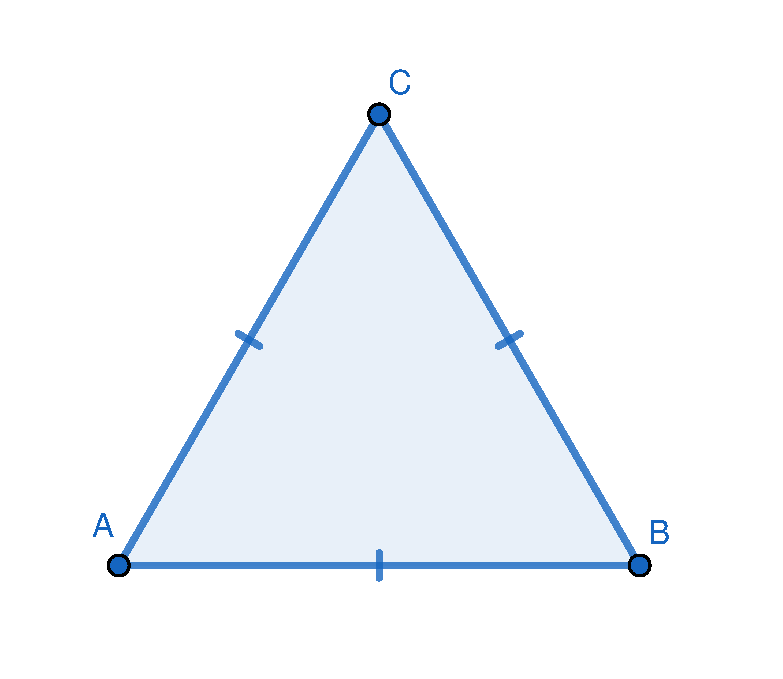
\includegraphics[height=5cm]{tex/chapter_1/assets/geogebra-export.pdf}
    \caption{Равносторонний треугольник}
\end{figure}
